\subsubsection{Reducing Computational Complexity}
Models of physical phenomena often begin with first principles, such as Newton's second law, Fourier's heat transfer equation, the Maxwell Equations, Schr\"odinger's equation, and the list continues. Terms in each equation are then expounded upon, incorporating other physical models of forces, energies, potentials, and more. The computational expense of a model is determined by how much physics is incorporated and the resolution at which the problem is modeled, among many other considerations. One workaround is better computers that can handle a larger I/O stream. Another approach is reduce the number of operations performed while still achieving a good enough description of the underlying physics.

Scientific endeavors are focused around descriptions of physical phenomena that are as accurate as possible. From an engineering and process modeling perspective, having a model that is `good enough' at modeling the phenomenon suffices. In this case, `good enough' means the model makes accurate predictions for the engineering application. Currently existing computational models can be downsized to be just `good enough' by analysis of which physics actually need to be incorporated to accurately predict the final result. 

A combinatorial approach can be employed to determine the most important inputs of a simulation by iterating through many possible manufacturing conditions and evaluating the difference in results. Many simulations can be run and then analyzed for conditions such as computation time or accuracy with experimental results. Similarly, running a test matrix of manufacturing conditions can also give insight to the \textit{best} conditions for a desired part property, like density. Kamath et al. applied a random forest algorithm to both of these ends. Their goal was to find the most important manufacturing conditions impacting melt pool depth and predict the best melt pool conditions to produce fully dense 316L stainless steel parts. To understand why Kamath's study was successful, it is necessary to understand the basics of random forest algorithms. 

Two key strengths of the random forest algorithm are its ease of use and its quick training time. Random forests are easy to use because they do not require tuning many hyper-parameters. Furthermore, random forests are very good at sifting through many irrelevant features to find the features that actually matter. They do not require data scaling or feature selection. Random forest training is also computationally inexpensive and easily parallelized. Random forests provide two advantages that are particularly important in the context of materials science: the ability to efficiently calculate uncertainty estimates and the added interpretability of feature importance metrics. Based on their ensemble nature, it is possible to generate uncertainty estimates for random forest predictions using jackknife-based procedures~\cite{Efron1992, Efron2014, Wager2014}. While uncertainty estimates are not needed in many mainstream machine learning use cases, they are critical in many materials science applications. Random forests also provide more interpretability than other machine learning methods. They automatically identify the most important features in a given model based on how often a feature is used in splitting criteria and what the aggregated information gain is over those splits. These feature importance metrics can provide insights into how the model is making its predictions. 

%\begin{figure}[t]
%\begin{center}
%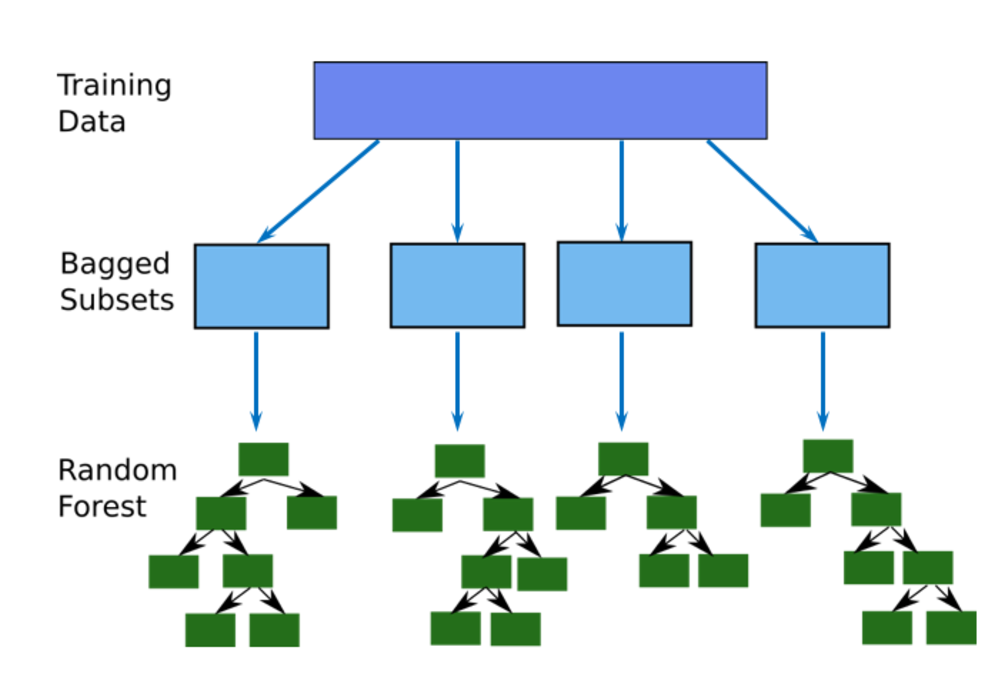
\includegraphics [width=65mm]{Images/randomforest2.eps}
%\end{center}
%\caption{Schematic of the random forest algorithm. The training data are randomly subsampled via bagging, and each bag is used to train a decision tree. All trees have an equal vote toward the final prediction.} 
%\label{fig:randomforest} 
%\end{figure}

Random forests have been applied successfully to a range of applications in materials science. They have been used to discover new Heusler compounds~\cite{Oliynyk2016} and new thermoelectric materials~\cite{Gaultois2016}. They have also been used to model material properties such as thermal conductivity in half-Heusler semiconductors ~\cite{Carrete2014} and to break down fields for dielectrics~\cite{Kim2016}. Ling et al.~\cite{Ling2017} demonstrated how random forest models with jackknife-based uncertainty estimates could be used for experimental design in materials science. The application of machine learning for experimental design is particularly compelling for AM, where there are many processing steps that affect build quality. 

Kamath utilized random forests among other machine learning techniques to predict melt pool depths based on the results of an Eagar--Tsai model for powder melting \cite{Kamath2016}. The Eagar--Tsai model uses a Gaussian laser beam incident on a metal substrate and models the temperature distribution throughout a bed of powder. Kamath was seeking to understand the most important laser parameters to use for predicting a melt pool's size and shape. Kamath started with the inputs of the Eagar--Tsai model and ordered them based on their numerical value. Then, a random forest algorithm was built that split variables based on the standard deviation of their associated output. The main idea was that variables that had a high impact would have a low standard deviation in their associated outputs. Using this method, they found that laser speed and power were the most important inputs for determining the melt pool depth and shape. After determining the most important inputs, the same regression tree was applied in order to find optimized manufacturing conditions for fully dense parts, using the same method.

Kamath's study also highlights a theme across studies of AM: the process combines separately known physics across separate domains. For example, a laser physics model will have a set of descriptors for describing the laser's behavior, while a solidification model will have a separate set of descriptors for itself. Descriptions across separately contained models do not obviously demonstrate how the descriptors interact, or which descriptors from one model are important to include in the other model. Science has long benefited from simple models, possibly empirical, which provide a small amount of physical descriptors to model specific properties. Machine learning algorithms can search through physical parameters used to model AM to find the lowest dimensional description which explains the widest swath of phenomenon. This is desirable for building computationally accessible models.

The many different computational models of AM, whether they are finite/direct element, central difference, phase field, or otherwise can all be upscaled to describe more and more physics.  Interaction potentials between forces during manufacturing can be added to models, requiring more input descriptors. Take, for example, a finite element model that describes thermal flux through a system from the interaction of a laser on a powder bed \cite{Khairallah2016}. There are many physics to consider here -- the energy transfer of the laser on the powder bed, movement of powder, phase change from powder to melt pool, thermal fluid mass transfer in the melt pool, convective, cooling, and radiative heat loss, and more. The full-physics model may have \textit{many} inputs $\mathbf{x} = (x_1,x_2,...,x_n)$ where $n$ is large.

The original, full-physics model produces a relationships $y = f(\mathbf{x})$ and may be computationally expensive, creating a bottleneck for process design and knowledge generation. A more computationally accessible model $y^*(\mathbf{x^*})$ would be desirable. In this case, the set of descriptors $\mathbf{x^*}$ consists of a subset of descriptors from $\mathbf{x}$, but is a much smaller set and requires less computational resources. 

Stated otherwise, the goal is to solve the objective function
\begin{equation}
	\text{min} ||y^*{(\mathbf{x^*})} - y(\mathbf{x})||
	\label{obj}
\end{equation}
such that $\{\mathbf{x^*} = \left(x_i...x_m\right) \in \mathbf{x} | m << n\}$

Finding the solution to Eqn, \ref{obj} can be achieved by fitting random sampling of descriptors from $\mathbf{x}$ and creating regression models on the outputs of the original model $y(\cdot)$. Presumably, the original full-physics model has been run and evaluated for accuracy. This means the researcher has a set of computationally-generated data $y$ as well as the inputs used to assess the model $\mathbf{x}$. 

Various subsets of the model inputs $\mathbf{x^*}_i$ can be chosen by randomly sampling the full list of inputs $\mathbf{x}$ repeatedly. Each subset of inputs can then be regressed upon, perhaps by using least squares regression
\begin{equation}
	\text{min} ||\mathbf{Y} - \mathbf{X^*_i} \mathbf{c_i}||
	\label{obj2}
\end{equation}
where $\mathbf{Y} = (y_1,y_2,...,y_n)$ are the outputs of the full-physics model, $\mathbf{X} = \left[ \mathbf{x^*} ,\mathbf{x^*},...,\mathbf{x^*}\right]^T$ is an $n \times m$ matrix of the subset of inputs, and $\mathbf{c}$ is a vector of weighting coefficients. This produces a randomly-generated model $y^*(\mathbf{x^*_i}) = \mathbf{X^*_i}\mathbf{c_i}$ which may or may not be able to accurately reproduce $y(\cdot)$. To find the \textbf{best} subset of inputs, one can solve 
\begin{equation}
	\underset{\mathbf{c}}{\text{min}}|| \mathbf{Y} - \mathbf{X^*_i} \mathbf{c_i}|| + \lambda||\mathbf{c_i}||
	\label{KRR}
\end{equation}
which is the objective equation for a machine learning method known as Kernel Ridge Regression (KRR). The idea behind Eqn. \label{KRR} is that it is a feasible minimization problem from a complexity perspective, i.e. it is convex. KRR is the basis of a descriptor set investigation performed by Ghiringhelli et al. to find the lowest dimensional descriptor for predicting crystal structure.They were able to identify one-dimensional, two-dimensional, and three-dimensional descriptors that were all shown to be the ``best'' combinations of descriptors out of any $n$-tuple \cite{Ghiringhelli2015}. Better physical descriptors are often found by combinatorial analysis of as many independent variables and dependent variables as possible. The `best' descriptors found experimentally are usually judged based on the amount of physics they are able to reproduce. Using descriptor analysis, as Ghiringhelli did, experimentalists can find the best descriptors as quickly as possible. Then, when trying to predict material properties in the future, researchers know which descriptors to use or combine.